\documentclass[zihao = -4,cn]{oucart}
\usepackage{algorithm}
\usepackage{algorithmic}
\usepackage{graphicx}
\usepackage{subfigure}
\usepackage{booktabs}

\title{隐私保护的分布式机器学习系统原型设计与实现}
\entitle{Prototype design and implementation of distributed machine learning system for privacy protection}
\author{曾趸}
\studentid{16090022049}
\advisor{高峰}
\department{信息科学与工程学院}{2016级计算机科学与技术}

\cnabstractkeywords{
基于神经网络的人工智能方法近年来取得巨大的成就, 但是人工智能技术往往是基于大数据,即大数据驱动的人工智能。 但是数据的匮乏在一定程度上限制了人工智能的发展,与此同时,数据源之间存在着难以打破的壁垒。一方面,人工智能所需数据来源广泛,遍及各领域,且各领域数据往往是以孤岛形式存在,整合各领域的数据也面临重重阻力。另一方面,随着大数据的发展,世界各国对用户数据隐私和安全管理也日趋严格。因此,要解决大数据的困境,就要保证数据隐私的同时,让机器学习系统高效和准确的利用各自的数据进行学习。我设计并实现了一个分布式机器学习系统的原型框架,使模型可利用多方数据信息协同学习,且保证了数据隐私安全以及无预测性能损失,并为研究者提供了可拓展的算法接口。在该框架基础上,实现了现有的分布式学习算法,并对其优点和局限性进行了分析和讨论。
}{
神经网络,分布式,隐私保护
}
\enabstractkeywords{
Artificial intelligence method based on neural network has accomplished great achievements in recent years, and artificial intelligence technology is often based on big data, that is, big data-driven artificial intelligence. But the lack of data often limits the development of artificial intelligence. At the same time, there are barriers between data sources that are hard to break. On the one hand, AI needs a wide range of data sources, covering all fields, and the data in all fields are often in the form of isolated islands, so integrating the data in all fields also faces many obstacles. On the other hand, with the development of big data, the privacy and security management of user data are increasingly strict in the world. Therefore, in order to solve the dilemma of big data, it is necessary to ensure the privacy of data, at the same time, let the machine learning system efficiently and accurately use their own data for learning. I designed a basic model of distributed machine learning system, which can use multi-party data for model collaborative training, at the same time, ensure the data privacy security and no prediction accuracy loss, and provide researchers with scalable algorithm interface. And in the experiment, I use the current commonly used neural network and data set to test the effectiveness of the system.
}{
neural network, distributed ML, privacy-preserving
}

\begin{document}

\makecover

\makesignature

\makeabstract

\thispagestyle{tableofcontents}  
\tableofcontents

\newpage
\pagenumbering{arabic}
\setcounter{page}{1} 
% 正文内容
% 建议使用 \input{<文件名>} 指令引用其他文件
\section{引言}
1956年,在由达特茅斯学院举办的一次会议上,计算机专家约翰·麦卡锡提出了“人工智能”一词。 1997年5月11日,IBM的计算机系统“深蓝”战胜了国际象棋世界冠军卡斯帕罗夫。2006年,Hinton在神经网络的深度学习领域取得突破\cite{hinton2006fast},人类又一次看到机器赶超人类的希望,也是标志性的技术进步。2016~2017年,AlphaGo战胜围棋冠军。至今为止,深度学习已经取得了令人瞩目的成就,但当前的人工智能发展仍然受到很多限制。AlphaGo使用了超过300,000场棋局数据训练,才取得如此成绩,由此可见,训练数据的质量和数量是影响学习模型泛化效果的一大重要因素。\par
在这个信息爆炸的时代,人类社会中存有大量有用的数据,但是将如此庞大的分散数据集合起来所需要的资源开销极大。与此同时,世界各国和企业对隐私数据的保护和管理方面的意识日渐加强,例如,欧盟于2018年5月提出的the General Data Protection Regulation (GDPR)\cite{voigt2017eu}旨在保护用户的个人隐私和数据安全。中国于2017年颁布的《中华人民共和国网络安全法》和《中华人民共和国民法通则》要求,互联网企业不得泄露或篡改其收集的个人信息,在与第三方进行数据交易时,必须确保拟议的合同遵守法律规定的数据保护义务。使得社会中的大量数据不能被合法的收集起来(如用户手机上的数据),并使数据源之间形成壁垒,且领域间的数据以孤岛形式存在。这些法规的建立,显然将有助于建立一个更具公民性的社会,但也将对人工智能目前常用的数据交易程序提出新的挑战。\par
现今,传统的人工智能学习方法往往是在单一机构下,使用已预处理好的大量数据训练模型,再将模型部署至应用。其中,数据的收集和预处理需要耗费大量的资源。诸多限制例如GDPR和《网络安全法》使得数据的收集和预处理面临诸多限制因素,如何在不违反相关法律法规、不泄露隐私的条件下,合理地利用处于数据孤岛状态的各方数据,训练出一个有效的模型,是现如今面临的问题和挑战。\par
本文基于Python和深度学习框架MXNet设计了一个分布式学习系统原型框架,提供了隐私保护、分布式部署、多方网络交流模块等功能,并为用户提供该方向算法研究的快速实现解决方案。\par
\section{神经网络}
深度神经网络从大量高维数据中提取复杂特征,并且利用这些特征建立一个输入-输出模型。其结构往往含有多隐含神经网络层,从而实现一个将高维度输入映射至低纬度输出的一个方法。在本文的实验方法中,主要面向神经网络的监督学习方法,即输入的数据带有正确的输出标签。而多层神经网络是最常见的学习网络架构\ref{fig:MLP}。\par

\begin{figure}[h]
	\centering %居中
	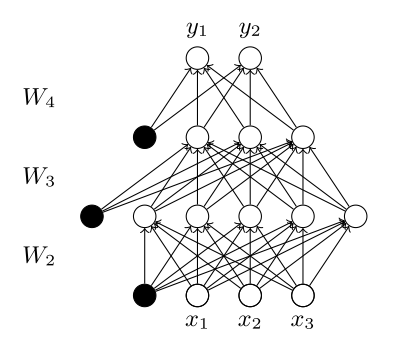
\includegraphics[width=8cm,height=7cm]{assets/MLP}
	\caption{多层感知机}
	\label{fig:MLP}
\end{figure}

在一个典型的多层网络中,每个神经元接收前一层神经元的输出信号$x$和一个特殊神经元发出的偏置信号$b$,然后计算其输入的加权平均$wx+b$,称为总输入。神经元的输出是通过对输入值应用非线性激活函数来计算的。神经网络第$k$层的输出$a_k = f(W_ka_{k-1})$,其中$f$为激活函数而$W_k$是决定每个输入信号贡献的权重矩阵。如果这个神经网络是一个分类模型,即将输入数据分类为有限个类(每个类由不同的输出神经元表示),那么最后一层神经网络的激活函数通常为softmax函数$f(z_j)=e^{z_j}\cdot(\sum_k{e^{z_k}})^{-1}$,$\forall{j}$。在这种情况下,最后一层的任意神经元$j$输出为输入数据是属于当前类$j$的相对概率。\par

\subsection{训练方法}
神经网络的学习是一个非线性函数的优化任务。在监督学习方面,目标函数是关于神经网络的输出和标签值的函数,描述了模型输出值与准确值之间的差异,模型的训练过程便是最小化目标函数的优化过程。\par
在神经网络的学习中,随机初始化神经元权值,作为梯度下降的起点。利用训练数据进行一次前向传播计算目标函数值,再反向传播计算每个神经元的梯度。以目标的负梯度方向调整神经网络权值,并作为下一次梯度下降的起点。重复上述过程,直到模型收敛或达到要求。关于神经网络的前向传播和反向传播计算细节可见\cite{周志华2016机器学习}。\par
随机梯度下降算法(SGD)将数据集拆分为多个批次,随机抽取一个批次来计算目标函数和梯度再调整参数,所以又称为MGBD(mini-batch gradient descent)。与标准的梯度下降法相比,随机梯度下降法在计算梯度时加入了随机因素,有机会在搜索过程中跳出局部最优。本文实验主要采用了随机梯度下降作为优化算法。\par
设$W$为神经网络的所有参数权值,特别的$W_j$为神经网络某一层的参数权值。$E$为训练的目标函数,$E$通常为$L^2$范数或者交叉熵\cite{murphy2012machine}。反向传播过程会计算目标函数E关于每一层权值的偏导,然后通过将权值减去梯度的方法更新参数。对于单层参数$W_j$的更新方法如下:\par
\begin{equation}
W_j := W_j - \eta \frac{\partial E_i}{\partial W_j} \label{eqa:grad}
\end{equation}
其中$\eta$是学习率,$E_i$是在数据集第i个小批量的目标函数结果。\par
综上关于神经网络的学习过程,简单的可以描述为:
\begin{itemize}
	\item [1)]
	随机初始化网络模型参数,作为模型迭代起点。
	\item [2)]
	利用训练数据集进行前向传播,计算目标函数函数。
	\item [3)]
	反向传播计算各层参数关于目标函数的梯度。
	\item [4)]
	根据式\ref{eqa:grad}以负梯度方向调整各层网络参数,回到步骤2),直至模型收敛或达到要求。
\end{itemize}
\par

\section{分布式学习}
大规模分布式机器学习系统为解决怎样协调和利用大量的GPU集群,来快速且高效地完成深度学习模型的训练任务并达到较好的收敛结果。 分布式机器学习在如何分配训练任务,调配计算资源,协调各个功能模块,以达到训练速度与精度的平衡方面,已经有了较为成熟的研究成果\cite{ho2013more}\cite{xing2015petuum}\cite{wei2015managed}。但是其主要是为了解决训练数据集太大或模型规模太大的问题,数据集仍然是集中于集群系统之中,传统的分布式学习便面临着数据收集和储存的成本问题,以及数据孤岛的限制。
\subsection{隐私保护的基本要求}
分布式学习中隐私保护的基本要求即为:在模型训练的过程中,本地数据自始至终不能离开本地。因此,可以将学习过程中的模型分为全局模型和本地模型,且本地模型与全局模型保持同步。数据持有方可利用本地数据对本地模型进行训练,反向传播得到的梯度信息或已更新地本地模型信息通过网络传至全局模型管理方,用于全局模型的更新,见示意图\ref{fig:commu}。
\begin{figure}[h]
\centering %居中
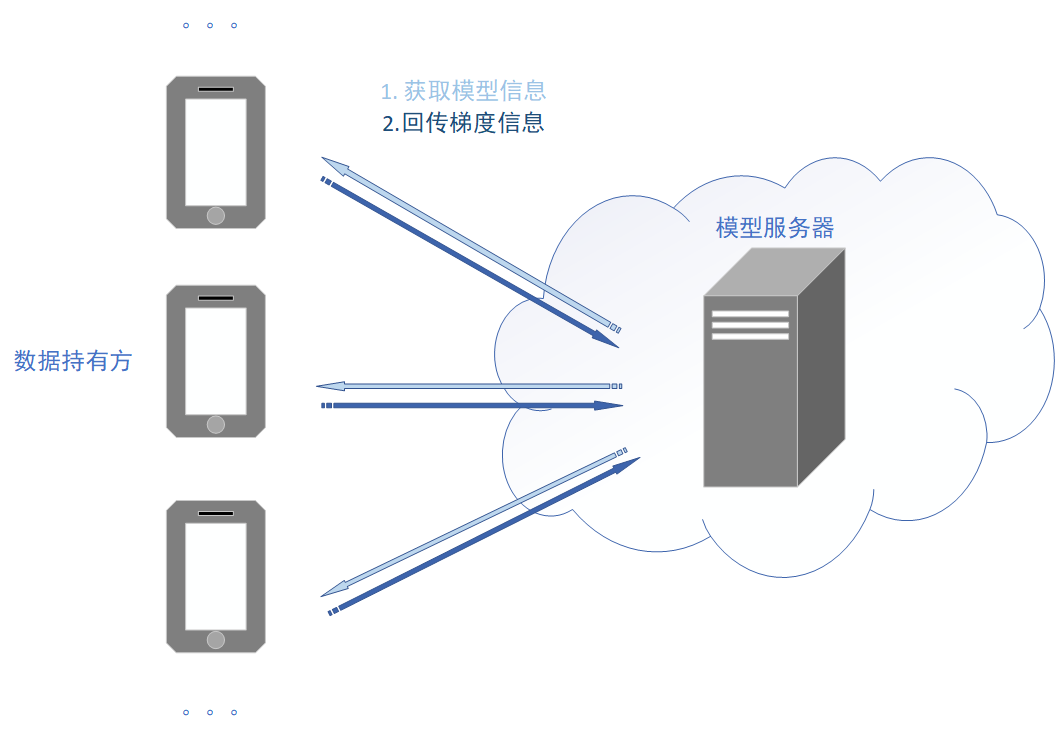
\includegraphics[width=15cm,height=9cm]{assets/test}
\caption{信息交流示意图}
\label{fig:commu}
\end{figure}

\subsection{学习系统架构简述}
基于参数服务器的通信拓扑结构是最为适合该学习算法的分布式系统架构。参数服务器的架构可以把参数服务器看做是一个媒介,在工作节点之间的媒介,负责数据交流,通信只发生在工作节点和参数服务器之间。\par
参数服务器负责管理全局模型,并维护与工作节点之间的通信和信息交流。工作节点即为数据的持有方,工作节点负责维护本地模型,并与参数服务器协同工作,合理利用本地数据更新全局模型。\par
为了描述方便,仅描述参数服务器与单个Client之间的算法流程关系。综合隐私保护的要求,即数据不能离开本地,与C/S架构的分布式系统,可将分布式学习过程抽象为:
\begin{itemize}
	\item [1)]
	参数服务器随机初始化全局模型$W^{(global)}$,工作节点与参数服务器通信获得模型$W^{(local)}$,特别的,$W^{(global)} = W^{(local)}$。
	\item [2)]
	工作节点利用本地数据执行模型的学习过程,并更新本地模型$W^{(local)}$。
	\item [3)]
	工作节点将本地训练的模型或梯度上传至参数服务器。
	\item [4)]
	参数服务器接收信息,并根据信息更新全局模型$W^{(global)}$。\par

	
\begin{figure}[h]
	\centering %居中
	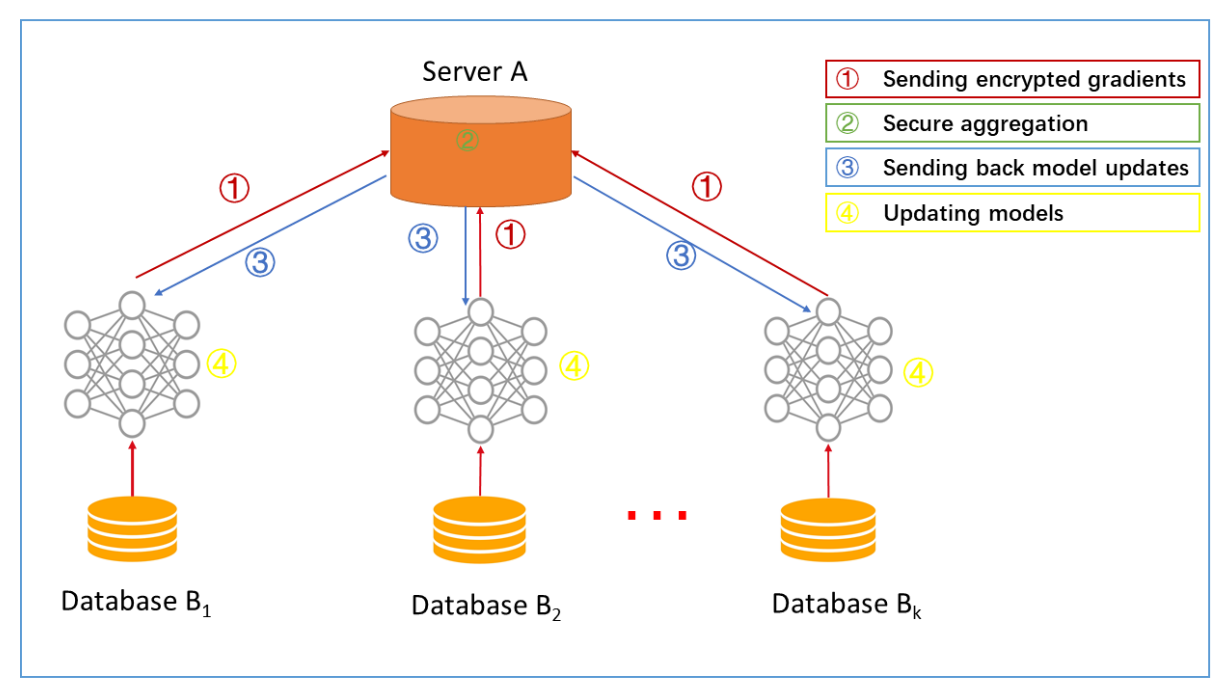
\includegraphics[width=12cm,height=7cm]{assets/fed}
	\caption{示意图,引用自论文\cite{yang2019federated}}
	\label{fig:MLP}
\end{figure}

\end{itemize}
\subsection{分布式最优化算法}
随机梯度下降(SGD)作为最优化算法多用于神经网络模型训练,通过优化目标函数取得了更好的效果。优化算法的设计仍然是该方向研究的热点问题之一,合理的优化算法可以在加速模型收敛的同时,达到较好的泛化效果。在这个方面,已经有很多优秀的工作成果,其中Federated Averaging(后称FedAvg)\cite{mcmahan2016communication}在通信带宽有限以及数据分布不均衡的学习场景下,在多种模型和场景下能高效地训练模型并收敛至目标准确率,而后将在我的系统框架下,开发并实现该算法,并对该算法的优点和局限性进行讨论,从而体现该框架的可用性。具体实验内容将在第五章讨论。

\subsubsection{Federated SGD}
在前文提到限制条件下,SGD算法仍可以自然的部署于分布式学习,本文称之为Federated SGD(后称FedSGD)。其分为Server和Client两部分,算法伪代码见\ref{FedSGDServer}。在我实现的框架中,其中Client端返回信息为模型或梯度取决于具体的算法。\par

%Server端算法
\begin{algorithm}[h]
	\caption{Federated SGD
		\\$w$为模型权重参数; $\eta$为模型的学习率; $l(w;b)$为目标函数。}
	\label{FedSGDServer}
	{\bfseries Server Excutes:}
	\begin{algorithmic}
		\STATE 初始化模型权重参数$w_0$
		\REPEAT
		\STATE 等待Client连接Server
		\IF{Client请求模型}
		\STATE 将模型参数下发至Clien
		\ELSIF{Client回传模型}
		\STATE 接收Client回传的模型$w_t$
		\STATE Server更新模型 $w_{t+1} := w_{t}$
		\ELSIF{Client回传梯度}
		\STATE 接收Client回传的梯度$\nabla{l(w;b)}$
		\STATE Server更新模型 $w_{t+1} := w_t - \eta\nabla(l(w;b))$
		\ELSE
		\STATE 非法连接
		\ENDIF
		\UNTIL{模型达到收敛条件}
	\end{algorithmic}
	%Client端算法
	{\bfseries Client Excutes:}
	\begin{algorithmic}
		\STATE 向Server请求模型参数$w_t$
		\FOR{batch $b \in B$}
		\STATE 更新模型 $w_t := w_t-\eta\nabla{l(w;b)}$
		\ENDFOR
		\STATE 返回模型$w_t$或梯度$\sum{\nabla{l(w;b)}}$至Server 
	\end{algorithmic}
\end{algorithm}

FedSGD属于同步算法,Server端面向多Client端进行模型学习时,Server需要等待当前Client完成任务并返回信息,且Server端将模型更新后才能进行下一轮的学习,使得FedSGD不适用于大规模学习,因为Server和大部分Client的时间用于等待,学习效率极低,其表现将在第五章讨论与分析。

%%Server端算法
\begin{algorithm}
\caption{Federated SGD
\\$w$为模型权重参数; $\eta$为模型的学习率; $l(w;b)$为目标函数。}
\label{FedSGDServer}
{\bfseries Server Excutes:}
\begin{algorithmic}
\STATE 初始化模型权重参数$w_0$
\REPEAT
\STATE 等待Client连接Server
\IF{Client请求模型}
\STATE 将模型参数下发至Clien
\ELSIF{Client回传模型}
\STATE 接收Client回传的模型$w_t$
\STATE Server更新模型 $w_{t+1} := w_{t}$
\ELSIF{Client回传梯度}
\STATE 接收Client回传的梯度$\nabla{l(w;b)}$
\STATE Server更新模型 $w_{t+1} := w_t - \eta\nabla(l(w;b))$
\ELSE
\STATE 非法连接
\ENDIF
\UNTIL{模型达到收敛条件}
\end{algorithmic}
%Client端算法
{\bfseries Client Excutes:}
\begin{algorithmic}
\STATE 向Server请求模型参数$w_t$
\FOR{batch $b \in B$}
\STATE 更新模型 $w_t := w_t-\eta\nabla{l(w;b)}$
\ENDFOR
\STATE 返回模型$w_t$或梯度$\sum{\nabla{l(w;b)}}$至Server 
\end{algorithmic}
\end{algorithm}
\subsubsection{Federated Averaging}
FedAvg算法在保证模型收敛的同时,降低了模型的更新轮次,降低了模型的收敛时间。FedAvg算法由3个主要参数控制:$C$,每一轮迭代计算中,参与的Client数占所有Client的比率;$E$,Client遍历本地数据集的次数,即epoch;$B$,Client训练时本地小批量数据的大小。特别的,当$C=0$时,即每一轮模型迭代只有一个Client参与,该算法退化为FedSGD。三个参数对Client间的并行计算,单Client计算量大小做出的要求,通过提高并行和单个Client的计算量,使得模型收敛更快,将在第五章讨论。\par
对于一个拥有数据集大小为$n_k$的Client,每一轮本地模型的更新次数由$u_k = E\frac{n_k}{B}$。算法伪代码可见\ref{FedAvg}。算法可描述为,每一个Client采用本地数据集计算并对模型进行一次迭代,Server将各Client取得的模型权重参数进行加权平均生成新模型,其中各Client的加权权重定义为其数据集大小占总数据集的比率(拥有更多数据的Client的模型更可信)。
%\renewcommand{\algorithmiccomment}[1]{// #1}
\begin{algorithm}[h]
\caption{Federated Averaging\\
Client总数为$K$且以$k$标志;$B$是本地数据批量大小;$E$是本地训练epoch;$\eta$是学习率。}
\label{FedAvg}
{\bfseries Server Excutes:}
\begin{algorithmic}
\STATE 初始化模型权重参数$w_0$
\FOR{每一轮 t}
\STATE $m \leftarrow \max(C\cdot K,1)$
\STATE $S_t$ $\leftarrow$ (随机选取Clients子集,其数量为m)
\FOR{每一个Client $k \in S_t$} 
\STATE $w_{t+1}^{k}\leftarrow$ClientUpdate($k$,$w_t$) \COMMENT{各Client间并行计算}
\ENDFOR
\STATE $w_{t+1}\leftarrow\sum_{k=1}^{K}\frac{n_k}{n}w_{t+1}^k$
\ENDFOR
\end{algorithmic}

{\bfseries ClientUpdate($k,w$):} // 在Client $k$上运行
\begin{algorithmic}
\STATE $\mathcal{B}$ $\leftarrow$ 将本地数据集以batch大小$B$分割
\FOR{每一个本地epoch $i$ 从1到$E$}
\FOR{batch $b \in \mathcal{B}$}
\STATE $w\leftarrow w-\eta\nabla{l(w;b)}$
\ENDFOR
\ENDFOR
\STATE 返回$w$至Server
\end{algorithmic}
\end{algorithm}


\begin{algorithm}[h]
	\caption{Federated Averaging\\
		Client总数为$K$且以$k$标志;$B$是本地数据批量大小;$E$是本地训练epoch;$\eta$是学习率。}
	\label{FedAvg}
	{\bfseries Server Excutes:}
	\begin{algorithmic}
		\STATE 初始化模型权重参数$w_0$
		\FOR{每一轮 t}
		\STATE $m \leftarrow \max(C\cdot K,1)$
		\STATE $S_t$ $\leftarrow$ (随机选取Clients子集,其数量为m)
		\FOR{每一个Client $k \in S_t$} 
		\STATE $w_{t+1}^{k}\leftarrow$ClientUpdate($k$,$w_t$) \COMMENT{各Client间并行计算}
		\ENDFOR
		\STATE $w_{t+1}\leftarrow\sum_{k=1}^{K}\frac{n_k}{n}w_{t+1}^k$
		\ENDFOR
	\end{algorithmic}
	
	{\bfseries ClientUpdate($k,w$):} // 在Client $k$上运行
	\begin{algorithmic}
		\STATE $\mathcal{B}$ $\leftarrow$ 将本地数据集以batch大小$B$分割
		\FOR{每一个本地epoch $i$ 从1到$E$}
		\FOR{batch $b \in \mathcal{B}$}
		\STATE $w\leftarrow w-\eta\nabla{l(w;b)}$
		\ENDFOR
		\ENDFOR
		\STATE 返回$w$至Server
	\end{algorithmic}
\end{algorithm}

\section{系统架构}
良好的系统架构使得系统具有高性能、高可用和可扩展性。该系统原型设计旨在为该方向研究者提供便捷的系统部署,即Server和Client的部署,并提供良好的网络通信策略,使研究者可以专注于算法的快速实现和想法的验证。\par
在系统架构层面,本文讨论的分布式学习系统需要广泛的点对点通信,即Server与Client之间的模型或梯度信息交流,因此,采取C/S架构是非常合理且自然的。我将该分布式学习系统分为Client端和Server端两个部分,并根据计算机网络分层思想将每个部分以功能划分为三层结构:网络层、逻辑层、计算层,见图\ref{fig:process}。其中计算层负责模型的维护,即模型定义,梯度计算,权值更新等功能,主要基于深度学习框架MXNet\cite{chen2015mxnet}实现。

\begin{figure}[h]
	\centering %居中
	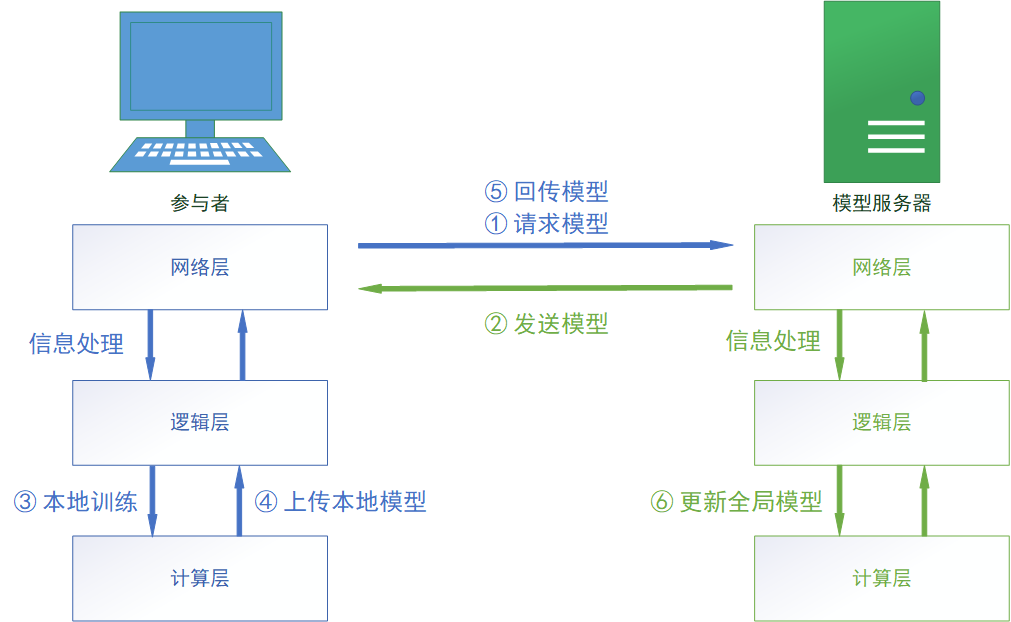
\includegraphics[width=14cm,height=8cm]{assets/process}
	\caption{架构示意图:箭头为信息流动情况,完整的一次模型更新过程为一个round}
	\label{fig:process}
\end{figure}

\subsection{网络层}
在本系统中,Server端与Client端需要可靠的网络通信用于传输信息,因此网络通信协议采用TCP协议,网络通信层负责维护Server端与Client端的网络通信状态,即TCP连接。\par
网络层的具体任务便是处理Server与Client的通信任务。Server端网络层主要负责处理来自Client端的请求信息,如模型参数请求或系统参数请求等,并将对应的响应任务下传至逻辑层,同时也需要处理逻辑层需要上传的信息发送任务。Client端网络层主要任务与Server端基本相同,区别主要体现在需要发送或接收的数据不同。\par
网络层为用户提供抽象的网络接口,如控制信息的接收与发送、模型或梯度信息的接收与发送。因此,用户只需要关注Client与Server间的数据交互关系和对应的逻辑处理,并将之送至下层。\par
\subsection{逻辑层}
现有的隐私保护的分布式学习算法研究,着重于网络通信优化和模型更新算法方向的探索。Deep Gradient Compression\cite{lin2017deep}方法在保证模型收敛的同时,大幅度降低了服务器与工作节点之间的通信资源消耗,论文中采用了多种方法,最核心的想法便是只传输重要的梯度信息来降低通信,可以简要概括为稀疏化更新。将梯度信息累积起来,知道当梯度值大于预设的阈值时,再将之发送至Server。Selective SGD\cite{shokri2015privacy}算法在使Client之间通过可靠的Server分享部分信息,使得Client端的训练结果更可靠,并使用户可在模型准确率与数据隐私强度之间权衡。这两种方法的核心思想均是在模型信息上下传递通信前后,对模型信息进行处理,与本文框架的分层架构相对应的即为逻辑层。\par
逻辑层作为网络层和计算层的中间层,负责处理上层往下传递的处理信号,以及处理计算层往上传递的计算结果,是整个系统架构的核心部分。逻辑层的可拓展性直接决定了框架的可拓展性。我开发的框架代码中,核心算法地实现与功能拓展均在逻辑中实现,为研究者提供了多种功能接口。\par
\subsection{计算层和架构总结}
MXNet是amazon的一个轻量化分布式可移植深度学习计算平台,在本文中用于计算层实现的核心框架。MXNet提供强大的模型定义和自动求导机制,为计算层的实现提供了很多便利。计算层在MXNet框架下实现了模型定义、数据加载、模型训练、梯度计算等功能,负责模型的基本计算与维护。\par
综合三层架构,本文的分布式学习系统可由三部分定义:通信算法、信息处理算法、模型,分别对应三层结构的用户自定义内容。框架为使用者提供了实现一个隐私保护的分布式系统需具备的基本功能模块。\par

\section{实验与分析}
本章在上述框架上开发一个基础的隐私保护的分布式学习系统,在其上拓展实现FedAvg算法并完成一个图像分类任务,讨论现有算法的优势与局限性。在体现框架可用性的同时,并分析未来的研究难点与方向。\par
实验中,我选择了常用的数据集MNIST,MNIST数据集包括60,000张图像的训练集和10,000张图像的验证集,每一张图片为0-9中的一个手写数字并带有标签。模型选取了简单的感知机模型(带有两个隐藏层,分别有128和64个神经元,并选取ReLu作为激活函数,下文称2NN)和卷积神经网络LeNet-5\cite{lecun2015lenet},在Mnist数据集上训练模型完成分类任务。在实验中我将训练数据集随机分割并分配至100个Client,每个Client有600张训练图。

\subsection{Federated SGD}
本节实验着重讨论FedSGD的表现。在实验中,着重比较在集中的数据集与分散的数据集上训练模型时,模型的泛化性能与计算量损耗之间的差别与关系。分布式训练的资源开销包括通信资源和计算资源,而集中数据集训练下仅有计算资源损耗,为了比较的方便,本节仅对计算资源的消耗进行讨论。\par
我定义对于单个数据在神经网络上做一次前向传播的计算量为$F$,一次反向传播的计算量为$B$。因此,一个模型的训练计算量可定义为$nF+mB$,其中$n$为前向传播次数,$m$为反向传播次数。例如,对于2NN以mini-batch大小为$b$,在数据集大小为$\mathcal{B}$,遍历训练$e$轮数据集,所消耗的计算量为:
\begin{equation}
\label{cal}
e(\mathcal{B}F_{mlp}+\frac{\mathcal{B}}{b}B_{mlp})
\end{equation}
\par
对于FedSGD,假设模型经过$n$轮通信完成训练,对于单轮训练的计算量可表示为$e_{client}(\mathcal{B}_{client}F+\frac{\mathcal{B}_{client}}{b}B)$,其中$\mathcal{B}_{client}$为本地数据集大小,则总计算量为$ne_{client}(\mathcal{B}_{client}F+\frac{\mathcal{B}_{client}}{b}B)$。\par
在我的实验中,分别取2NN和LeNet-5模型在验证集上的准率在97\%和99\%时的计算量作为基准,即模型在训练过程中,在验证集上准确率第一次超过预设准确率时的计算量。FedSGD在单轮迭代中,我设置Client的训练轮数$E=5$,且有$|\mathcal{B}_{Client}|=\frac{|\mathcal{B}|}{100}$,并由\ref{cal},可得在实验中,分布式训练与集中式训练的计算量关系式:
\begin{equation}
\frac{ne_{client}}{100}(\mathcal{B}F+\frac{\mathcal{B}}{b}B) = ne_{client}(\mathcal{B}_{client}F+\frac{\mathcal{B}_{client}}{b}B)
\end{equation}
因此,分别取集中式训练时的遍历数据集轮数$e$和分布式训练时的$\frac{ne_{client}}{100}$作为计算量对比数据,通过实验得表\ref{tab:experiment}。\par
%实验数据表格
\begin{table}[!htbp] 
\caption{\label{tab:experiment}数据集中式与分布式计算量对比}
\begin{tabular}{ccccccccc} 
\toprule 
\textbf{2NN} & \multicolumn{4}{c}{集中式训练} & \multicolumn{4}{c}{分布式训练,$E$=5}\\ 
学习率$\eta$ & $B$=200 & $B$=100 & $B$=50 & $B$=10 & $B$=200 & $B$=100 & $B$=50 & $B$=10 \\
\midrule 
0.01 & 84 & 41 & 23 & 6 & 83.3 & 43 & 23.55 & 7.55 \\ 
0.02 & 43 & 21 & 11 & 3 & 43 & 23.55 & 13.2 & 5.75 \\ 
0.04 & 21 & 11 & 6  & 3 & 23.55 & 14.4 & 10.2 & 5.35 \\ 
\bottomrule
\textbf{LeNet-5} \\
\hline
0.01 & 132 & 66 & 29 & 11 & 127.75 & 91.5 & 36.5 & 13.55 \\ 
0.02 & 54 & 27 & 18 & 4 & 71.5 & 35.5 & 26.65 & 11.75 \\ 
0.04 & 34 & 13 & 11 & 6 & 45.5 & 36.2 & 12.45 & 11.8 \\ 
\hline
\end{tabular}
\footnotesize
\qquad 实验中,不同参数的初始学习模型均为相同的随机初始化的模型,即迭代起点相同。
\end{table}
通过对比\ref{tab:experiment}中的实验数据可得,FedSGD在各个参数下的计算量相比于数据集中式训练,在达到相同准确率时,FedSGD均有不同程度的计算量损失,因为在被分割且数据不平衡的数据集上训练,需要通常更多次的迭代才能收敛到最优。此外,分布式计算需要额外的通信资源开销,且FedSGD在实际训练中,Server与部分Client大部分时间都花在等待当前Client模型训练。完成模型训练的时间代价过大,是该算法的主要问题。

\subsection{Federated Averaging}
在关于FedAvg的实验中,着重关注FedAvg方法对FedSGD算法的提升,即模型更新轮次。实验中,固定学习率$\eta$=0.04,Client训练轮数$E$=5,仍然取模型2NN和LeNet-5第一次在验证集上达到准确率97\%和99\%作为基准线,比较FedAvg在迭代轮次上,性能的提升。实验数据见\ref{tab:expFedAvg},其中$C=0.0$即为FedSGD,数据为Server端模型收敛至目标准确率所经过的迭代轮次$T$。\par

\begin{table}[!htbp]
\caption{\label{tab:expFedAvg}FedAvg与FedSGD实验结果数据。实验初始化模型与5.1节中的实验相同。}
\begin{center}
\begin{tabular}{ccccc}
\toprule
 & \multicolumn{2}{c}{\textbf{2NN}} & \multicolumn{2}{c}{\textbf{LeNet-5}} \\
$C$ & $B$=10 & $B$=100 & $B$=10 & $B$=100 \\
\midrule
0.0 & 107 & 288 & 236 & 724 \\
0.1 & 28(3.8$\times$)  & 99(2.9$\times$)  & 82(2.9$\times$)  & 80(9.1$\times$)  \\
0.2 & 34(3.1$\times$)  & 99(2.9$\times$)  & 51(4.6$\times$)  & 90(9.0$\times$)  \\
0.5 & 38(2.8$\times$)  & 101(2.9$\times$) & 49(4.8$\times$)  & 114(6.4$\times$) \\
1.0 & 35(3.1$\times$  )& 102(2.8$\times$) & 38(6.2$\times$)  & 134(5.4$\times$) \\
\bottomrule
\end{tabular}
\end{center}
\end{table}

参数$C$决定了系统Client端并行训练的强度,$C$越大,越多的Client同时参与一轮的计算。通过实验数据的纵向比较,对于不同的参数$C$,FedAvg算法性能的表现差别不大。参数$B$和$E$决定了Client在单次训练任务的计算量,通常情况下$E$与计算量成正相关,而$B$与计算量成负相关。根据实验数据的横向对比,在\textbf{2NN}和\textbf{LeNet-5}模型下,单机计算量的提升,相应对模型收敛速度有所提升。\par
综合实验结果分析,FedAvg相比于FedSGD在模型训练上表现更好,均有不同程度的速度的提升,提升效果取决于系统参数和模型解空间的协同效果。对于Client而言,在相同参数$B$和$E$下,FedAvg算法的计算量更大:$CK$为单轮迭代参与者数量,$T$为收敛迭代轮次,FedSGD算法下单轮迭代参与者数量为1,而FedAvg参与着数量远大于FedSGD,因此$TCK$即为FedAvg算法在Client端的计算量负载。实验中$K=100$,则FedAvg在Client端的计算量消耗远大于FedSGD。\par
FedAvg相比与FedSGD实质上是计算量与训练时间的权衡,FedAvg通过将模型训练过程并行化,并付出更多的计算资源获得了更短的训练时间。在实际应用场景中,人们往往希望模型训练时间更短,而不关心实际花费的计算量,因此FedAvg算法在实际的分布式训练场景中仍有用武之地。

\section{总结与展望}
本文设计并实现了一个隐私保护的分布式机器学习框架原型,该框架采用三层架构设计,并为研究者提供了分布式系统的算法实现的快速解决方案。之后,我基于该框架实现了Mnist数据集的图像分类任务学习的分布式学习算法,并拓展研究了FedAvg和FedSGD的实验,讨论了其各项表现。\par
将隐私保护的分布式系统部署在智能手机上是该方向的应用场景之一,在数据孤岛问题下,如果设计分布式学习算法使得多个数据持有方,在数据不平衡的情况下,保证数据隐私安全的同时,能协同有效的训练模型,仍然是一个重要的研究点。此外,对于系统鲁棒性的提升,即如何处理不稳定的参与者、对外部攻击的防御、恶意参与者的检测与防范仍是该方向的重要课题。

\newpage
%\bibliographystyle{unsrt}
\bibliography{refer}

\newpage
\begin{center}
\zihao{3} \textbf{致谢} \\
\end{center}

\newpage
\begin{center}
\zihao{3} \textbf{附录} \\
\end{center}
\end{document}
